\section{Results and Discussion}\label{sec:results}
The experiments in this section are used to compare the performance of \AlgName{} against a base-line co-kriging algorithm and an implement ion of the \motos{} framework, as described in Section~\ref{sec:exp}. Test suite $A$ is taken from~\cite{lv2021multi} and demonstrates the performance of \AlgName{} on a variety of problems with different sizes; while test suite $B$ is used to investigate the effect of problem size and error type. The results from each set of experiments are presented in a table with plots comparing the convergence of \AlgName{} and the base-line co-kriging algorithm on a representative sample of the problem instances. \motos{} is not included in the convergence plots as decisions are made \emph{a priori} and it is not an iterative process.

A summary of the results, their implications and statistical significance is also provided at the end of this section.

\subsection*{Test suite A}

Table~\ref{tab:results-a} presents the results from 30 runs of \AlgName{}, the base-line co-kriging algorithm and \motos{} on test suite $A$. In this table, it can be seen that \AlgName{} performs better than \motos{} for all instances. It also performs as well as or better than the base-line co-kriging algorithm with a few exceptions. For the tests on instances $f11$, $f14$ and $f16$, the base-line co-kriging algorithm was able to find at least one solution that was better than the best solution produced by \AlgName{}, and for the instances $f10$ and $f14$ it produced better solutions on average. In all of these instances, the differences between the algorithms are small, with both performing very similarly; whereas \AlgName{} outperforms the co-kriging by some margin in a lot of the other instances.

\begin{table*}[h!]
\centering
\caption{Results on dataset $A$ comparing \AlgName{} to \motos{} and the base-line co-kriging algorithm. Given are the number of decision variables ($D$), the square of the Pearson correlation coefficient ($r^2$), the best objective obtained, the mean best objective over the full set of runs ($\mu$) and the corresponding standard deviation ($\sigma$).}\label{tab:results-a}
\begin{adjustbox}{width=0.9\textwidth}
\begin{tabular}{lrrrrrrrrrrr} \toprule
& & & \multicolumn{3}{c}{Co-kriging} & \multicolumn{3}{c}{\motos{}} & \multicolumn{3}{c}{\AlgName{}}\\
\cmidrule(lr){4-6} \cmidrule(lr){7-9} \cmidrule(lr){10-12} 
Instance & $D$ & $r^2$ &\multicolumn{1}{c}{best}&\multicolumn{1}{c}{\(\mu\)} & \multicolumn{1}{c}{\(\sigma\)}&\multicolumn{1}{c}{best}& \multicolumn{1}{c}{\(\mu\)}&\multicolumn{1}{c}{\(\sigma\)}&\multicolumn{1}{c}{best}& \multicolumn{1}{c}{\(\mu\)}&\multicolumn{1}{c}{\(\sigma\)}\\ \midrule
%
$f10$ & 3 & 0.64 & \best{0} &  \best{2.2960}  &  3.5445         &   4.9076 &   29.6201 &   33.3903 &   \best{0} & 3.9189 &  5.3296\\
$f11$ & 3 & 0.74 &   \best{0.0001} &  0.0110  &  0.0077         &   0.0199 &    0.2043 &    0.1710 &  0.0004 &   \best{0.0098} &  0.0064\\
$f12$ & 4 & 0.79 & -8.1107 &  -3.8007 &  1.3426                 &  -3.8370 &   -1.7674 &    0.7283 &  \best{-9.5783} & \best{-5.8853}  &  1.5123\\
$f13$ & 4 & 0.89 &   0.6290 &  4.9366  &  5.0965                &  14.0887 &  159.2747 &  180.3111 &  \best{0.0519} &   \best{0.3457} &  0.1971\\
$f14$ & 5 & 0.75 &   \best{0.2509} &  \best{0.2583}  &  0.0039  &   0.2815 &    0.4025 &    0.0605 &  0.2522 &   0.2607 &  0.0037\\
$f15$ & 6 & 0.78 & 104.2304 &  1700.28 &  2015.04               & 894.6061 & 6069.7722 & 4689.5802 & \best{24.6278} & \best{152.9817} &144.6451\\
$f16$ & 8 & 0.82 & \best{7.3904}   &  196.810 &  171.7771       & 152.3790 &  502.9491 &  261.0805 &  7.9240 &  \best{75.2898} & 59.3423\\
$f17$ & 8 & 0.79 & -2.5859  &  42.0074 &  153.4414              &  87.9290 &  293.7373 &  104.7241 & \best{-3.0161} & \best{-2.8355} & 0.0967\\
%
\bottomrule
\end{tabular}
\end{adjustbox}
\end{table*}

This is supported by the convergence plots in Figure~\ref{fig:set-a-conv}. Here, it is clear that when the size of the problem is small, the performance of the two algorithms is very similar, with similar convergence rates; but as the size increases, both the average performance, and convergence rate, of \AlgName{} over co-kriging improves significantly --- with the most marked improvement being for problem $f17$. 

% \begin{figure*}[t]
%   \centering
%   \subfloat[$f11\ (D=3)$\label{fig:f11-conv}]{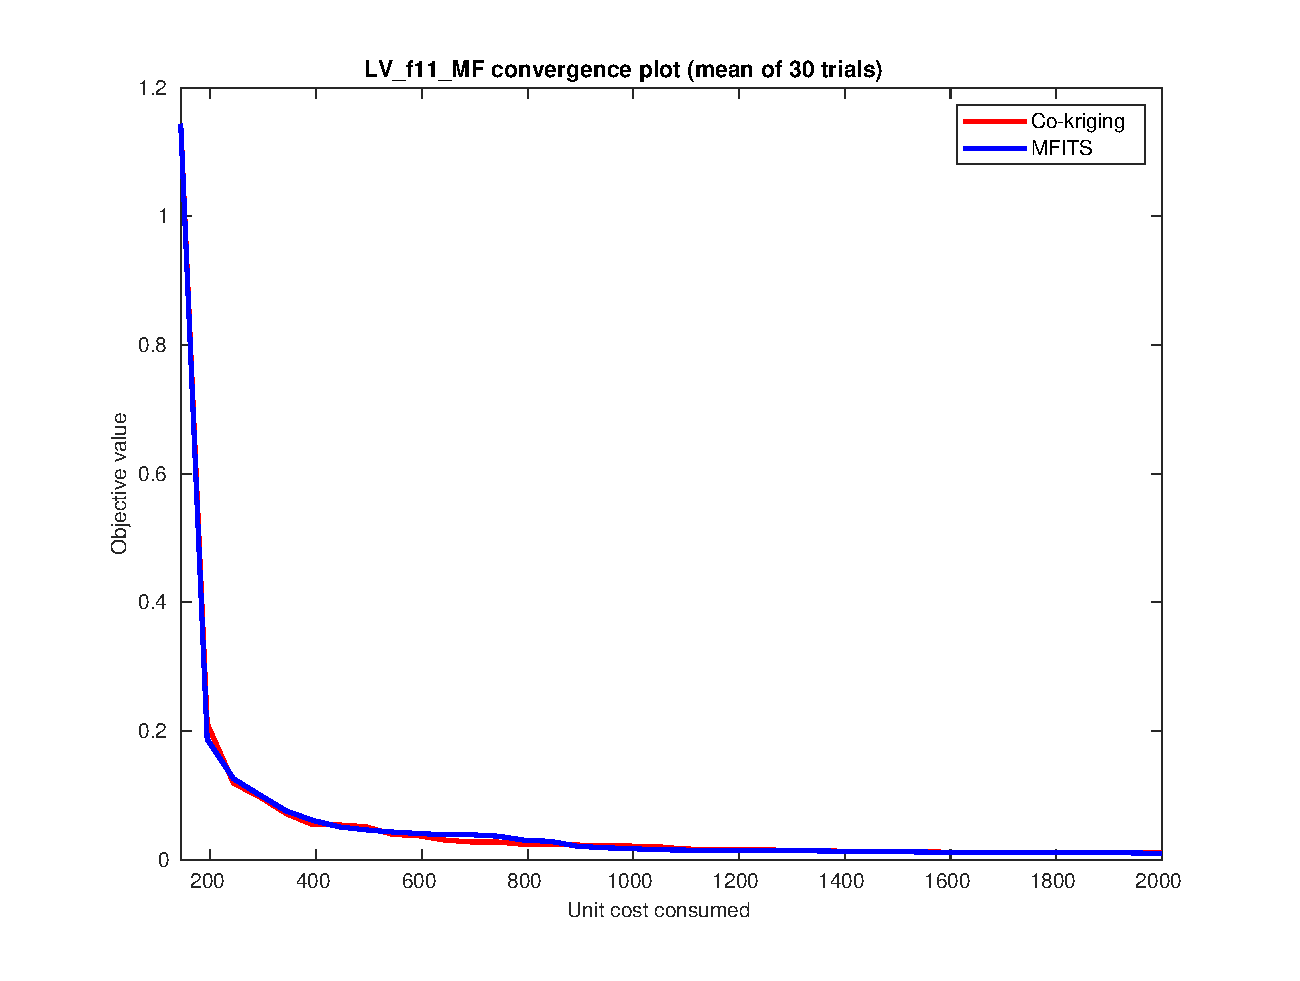
\includegraphics[width = 0.33\textwidth]{img/LV_f11_MF_conv_mean.eps}}
%   \subfloat[$f13\ (D=4)$\label{fig:f13-conv}]{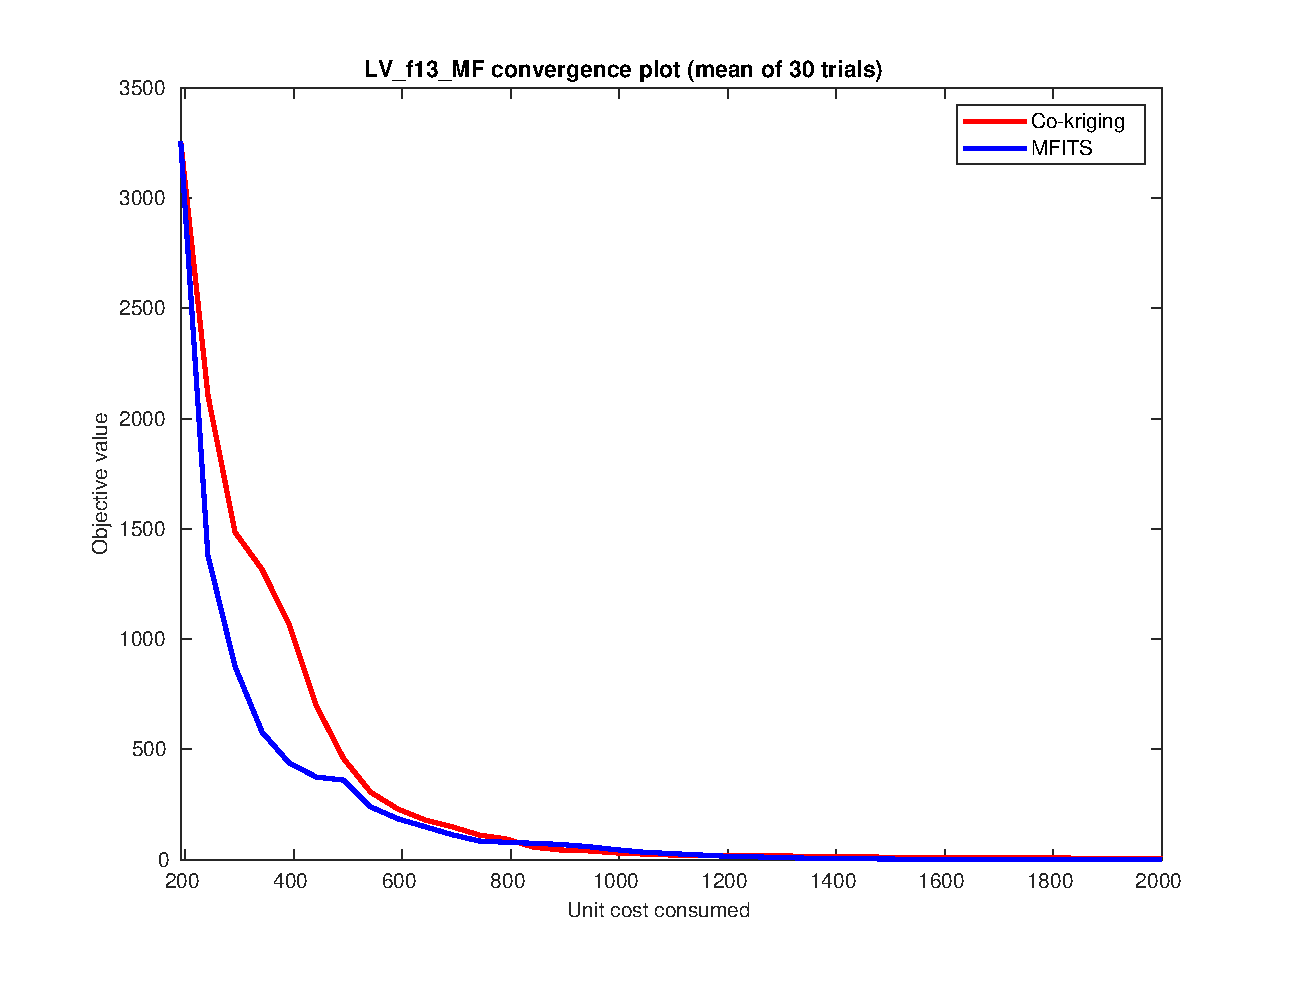
\includegraphics[width = 0.33\textwidth]{img/LV_f13_MF_conv_mean.eps}}
%   \subfloat[$f14\ (D=5)$\label{fig:f14-conv}]{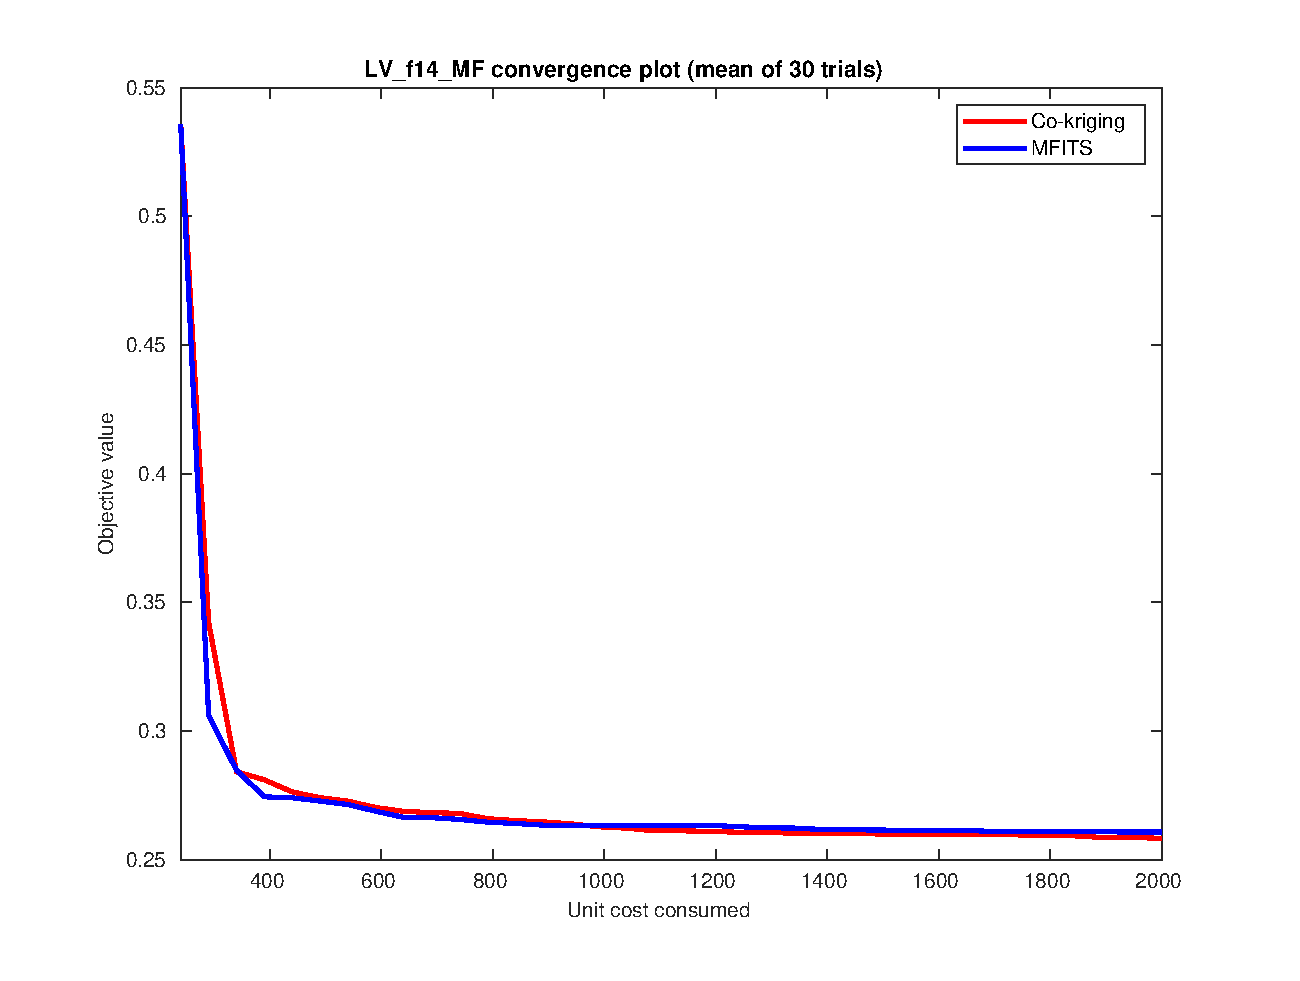
\includegraphics[width = 0.33\textwidth]{img/LV_f14_MF_conv_mean.eps}}\\
%   \subfloat[$f15\ (D=6)$\label{fig:f15-conv}]{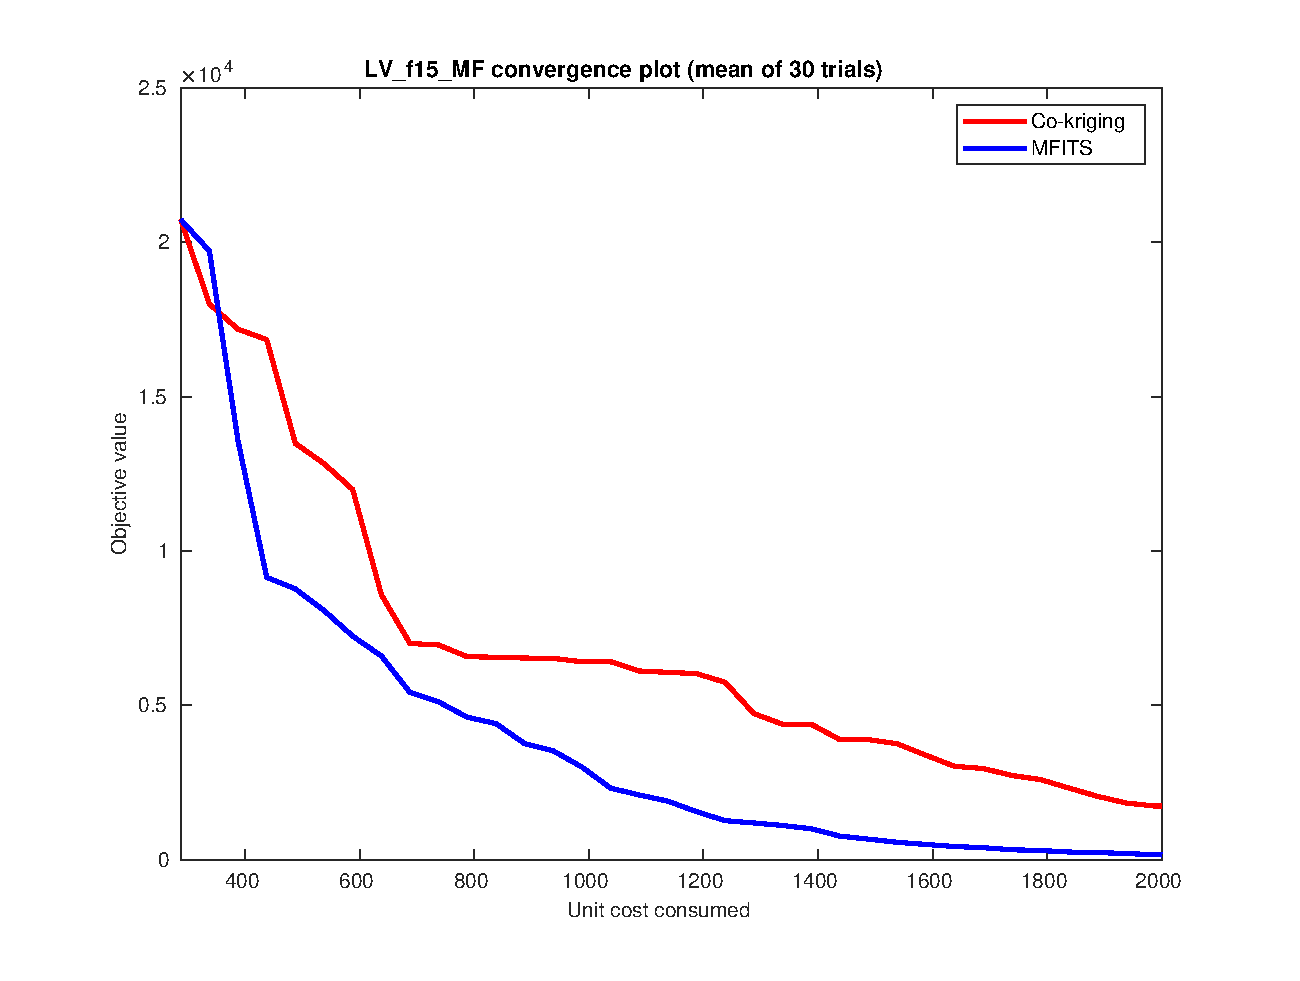
\includegraphics[width = 0.33\textwidth]{img/LV_f15_MF_conv_mean.eps}}
%   \subfloat[$f16\ (D=8)$\label{fig:f16-conv}]{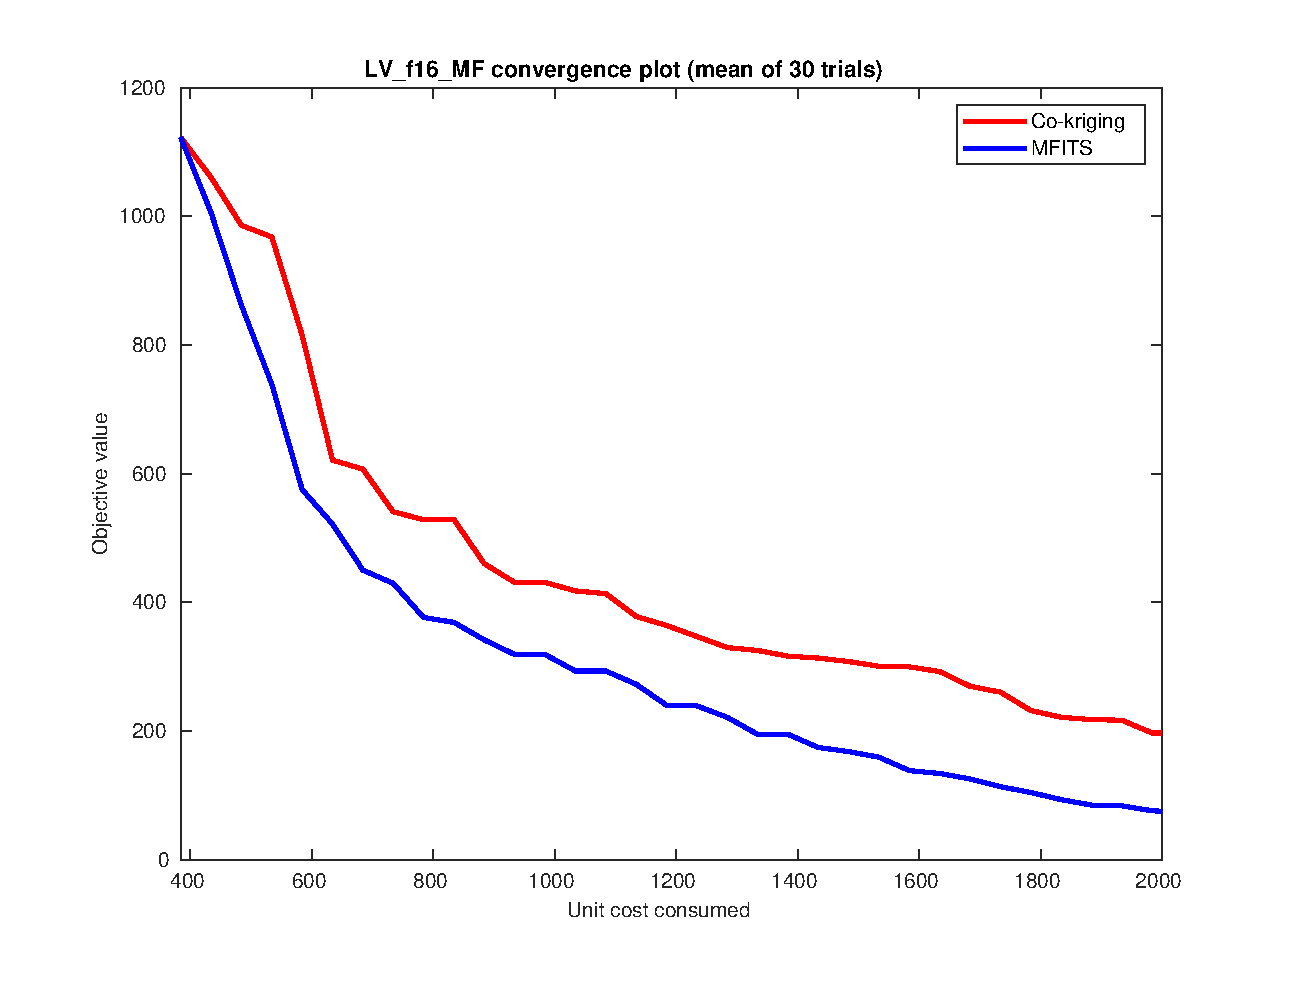
\includegraphics[width = 0.33\textwidth]{img/LV_f16_MF_conv_mean.eps}}
%   \subfloat[$f17\ (D=8)$\label{fig:f17-conv}]{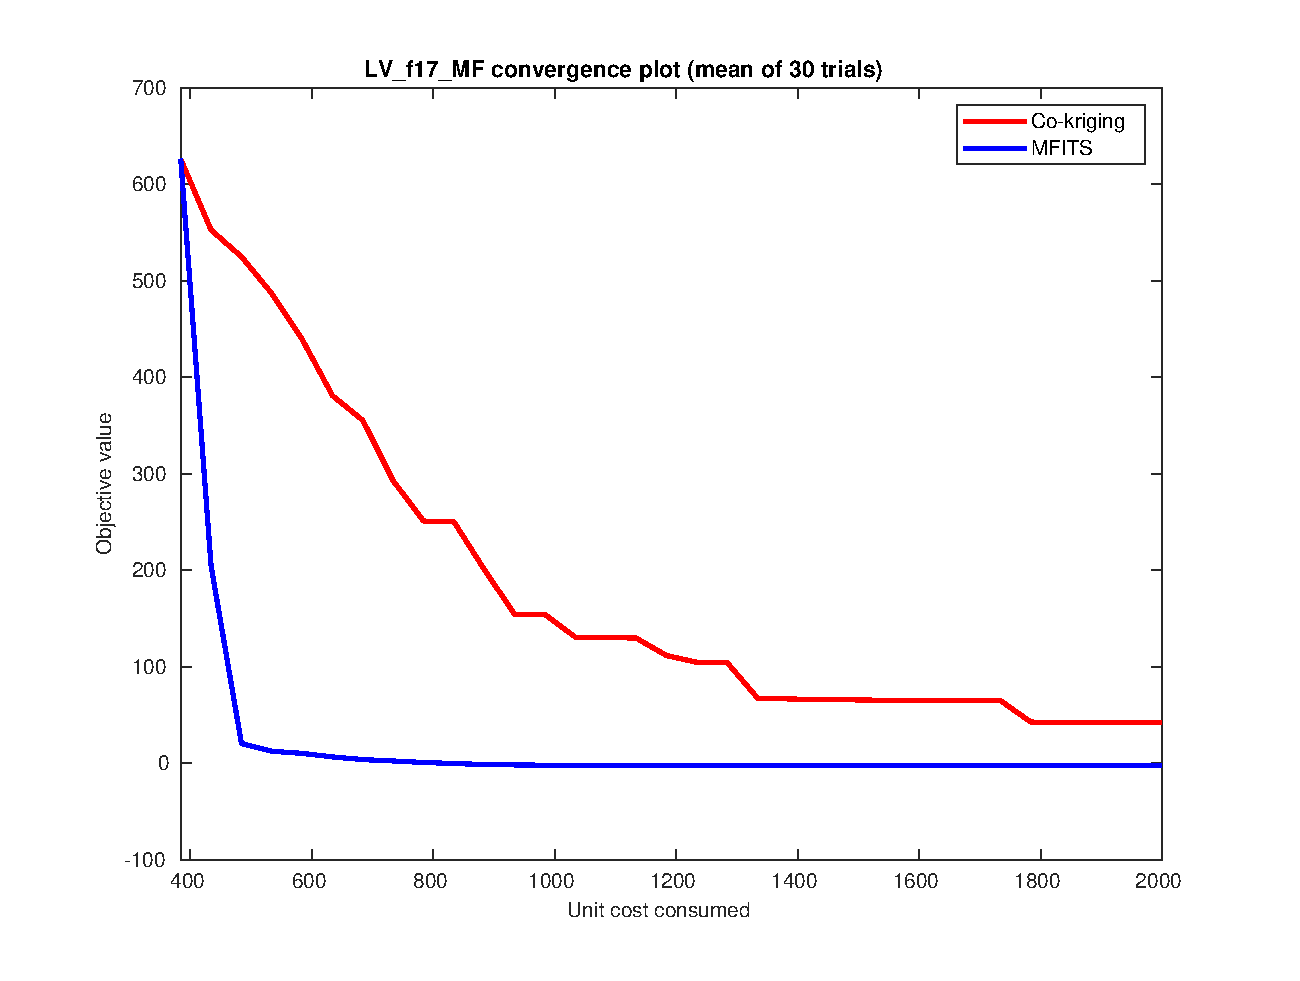
\includegraphics[width = 0.33\textwidth]{img/LV_f17_MF_conv_mean.eps}}
%   \caption{Mean convergence plots for problem instances $f11$, $f13$, $f14$, $f15$, $f16$ and $f17$ of dataset $A$, over 30 runs. \angus{will do pgfplots version}} 
%     \label{fig:set-a-conv}
% \end{figure*}
\begin{figure*}[t]
  \centering
  \subfloat{\includegraphics{plots/obj_label.tikz}}%
  \addtocounter{subfigure}{-1}%
  \subfloat[$f11\ (D=3)$\label{fig:f11-conv}]{\includegraphics[width = 0.28\textwidth]{plots/mfits/Lv_f11_plot.tikz}}
  \subfloat[$f13\ (D=4)$\label{fig:f13-conv}]{\includegraphics[width = 0.28\textwidth]{plots/mfits/Lv_f13_plot.tikz}}
  \subfloat[$f14\ (D=5)$\label{fig:f14-conv}]{\includegraphics[width = 0.28\textwidth]{plots/mfits/Lv_f14_plot.tikz}}\\
  \subfloat{\includegraphics{plots/obj_label.tikz}}%
  \addtocounter{subfigure}{-1}%
  \subfloat[$f15\ (D=6)$\label{fig:f15-conv}]{\includegraphics[width = 0.28\textwidth]{plots/mfits/Lv_f15_plot.tikz}}
  \subfloat[$f16\ (D=8)$\label{fig:f16-conv}]{\includegraphics[width = 0.28\textwidth]{plots/mfits/Lv_f16_plot.tikz}}
  \subfloat[$f17\ (D=8)$\label{fig:f17-conv}]{\includegraphics[width = 0.28\textwidth]{plots/mfits/Lv_f17_plot.tikz}}
  \caption{Mean convergence plots for problem instances $f11$, $f13$, $f14$, $f15$, $f16$ and $f17$ of dataset $A$, over 30 runs. Blue and red colours indicate \AlgName{} and the co-kriging baseline, respectively.} 
    \label{fig:set-a-conv}
\end{figure*}

\subsection*{Test suite B}
The purpose of test suite$B$ was to observe the effect of problem size on the performance of \AlgName{}, and to do so using two different error functions to ensure the results obtained are consistent and not over-fitted to a particular type of simulation error model. The results in Table~\ref{tab:results-b} compare the performance of \AlgName{}, \motos{} and the baseline co-kriging algorithm over 30 independent runs on the instances of test suite $B$. This suite comprises two problem instances from the literature, with variable dimensionailty, using error functions $e_2$ and $e_6$ as described in~\cite{wang2017generic}.

\begin{table*}[h!]
\centering
\caption{Results on Griewank and Michalewicz test problems using Wang error functions 2 and 6 (indicated by subscript), comparing \AlgName{} to \motos{} and the base-line co-kriging algorithm. Given are the number of decision variables ($D$), the square of the Pearson correlation coefficient ($r^2$), the best objective obtained, the mean best objective over the full set of runs ($\mu$) and the corresponding standard deviation ($\sigma$).}\label{tab:results-b}
\begin{adjustbox}{width=0.9\textwidth}
\begin{tabular}{lrrrrrrrrrrr} \toprule
& & & \multicolumn{3}{c}{Co-kriging} & \multicolumn{3}{c}{\motos{}} & \multicolumn{3}{c}{\AlgName{}}\\
\cmidrule(lr){4-6} \cmidrule(lr){7-9} \cmidrule(lr){10-12} 
Instance & $D$ & $r^2$ &\multicolumn{1}{c}{best}&\multicolumn{1}{c}{\(\mu\)} & \multicolumn{1}{c}{\(\sigma\)}&\multicolumn{1}{c}{best}& \multicolumn{1}{c}{\(\mu\)}&\multicolumn{1}{c}{\(\sigma\)}&\multicolumn{1}{c}{best}& \multicolumn{1}{c}{\(\mu\)}&\multicolumn{1}{c}{\(\sigma\)}\\ \midrule
%
$Griewank_{2}$    & 3 & 0.73 & \best{0} &  \best{0.0018} &  0.0083 &    0.0019 &    0.0735 &    0.0440 & \best{0} &   0.0072 &  0.0137\\
                  & 5 & 0.54 & \best{0} &  0.0535 &  0.0723        &    0.1428 &    0.3886 &    0.1245 & \best{0} &   \best{0.0485} &  0.1055\\%
                  & 8 & 0.37 & \best{0} &  0.6538 &  0.3363        &    0.5606 &    0.8036 &    0.1100 & \best{0} &   \best{0.1864} &  0.2531\\
$Griewank_{6}$    & 3 & 0.74 & \best{0} &  \best{0.0056} &  0.0114 &    0.0076 &    0.0564 &    0.0290 & \best{0} &   0.0104 &  0.0130\\
                  & 5 & 0.76 & \best{0} &  0.0730 &  0.1145        &    0.1139 &    0.3792 &    0.1328 & \best{0} &   \best{0.0361} &  0.0778\\
                  & 8 & 0.76 & \best{0} &  0.4560 &  0.4238        &    0.5565 &    0.8108 &    0.1249 & \best{0} &   \best{0.2089} &  0.3539\\
\midrule  
$Michalewicz_{2}$ & 3 & 0.77 &  -2.7239 & -2.3582 &  0.2587        &   -2.4612 &   -1.8939 &    0.2366 & \best{-2.7360} &  \best{-2.5305} &  0.1557\\
                  & 5 & 0.73 &  -3.5164 & -2.9470 &  0.2921        &   -3.2841 &   -2.4554 &    0.3928 & \best{-3.5653} &  \best{-2.9953} &  0.3219\\%
                  & 8 & 0.64 &  -4.1813 & -3.0214 &  0.4958        &   -4.2150 &   -3.0818 &    0.4406 & \best{-4.5542} &  \best{-3.3046} &  0.5004\\
$Michalewicz_{6}$ & 3 & 0.76 &  -2.7194 & -2.2412 &  0.2978        &   -2.4657 &   -1.8847 &    0.2927 & \best{-2.7409} &  \best{-2.4080} &  0.2711\\
                  & 5 & 0.83 &  \best{-3.6198} & -2.6695 & 0.3986  &   -3.2980 &   -2.5380 &    0.3328 & -3.5511 &  \best{-2.9944} &  0.3490\\
                  & 8 & 0.86 &  -3.9978 & -3.1032 &  0.4929        &   -3.9627 &   -3.1363 &    0.3772 & \best{-4.2922} &  \best{-3.1672} &  0.4865\\
%
\bottomrule
\end{tabular}
\end{adjustbox}
\end{table*}

Again, the table shows that \AlgName{} outperforms \motos{} in all instances and the co-kriging baseline algorithm, with a few exceptions. For the Michaelwicz problem using error function $e_6$ and with the problem instantiated with five decision variables, the co-kriging base-line algorithm managed to find the best over-all solution. However \AlgName{} still performed better on average. The only time when the co-kriging base-line outperformed \AlgName{} on average was on the two smallest instantiations of the Griewank problem. The convergence plots in Figures~\ref{fig:gw23-conv} and~\ref{fig:gw63-conv} show that the difference between the performance of both algorithms for these instances is reasonably negligible. The remaining plots in Figure~\ref{fig:set-b-conv} agree with the observations for test suite $A$.

% \begin{figure*}[h!]
%   \centering
%   \subfloat[$Griewank_2\ (D=3)$\label{fig:gw23-conv}]{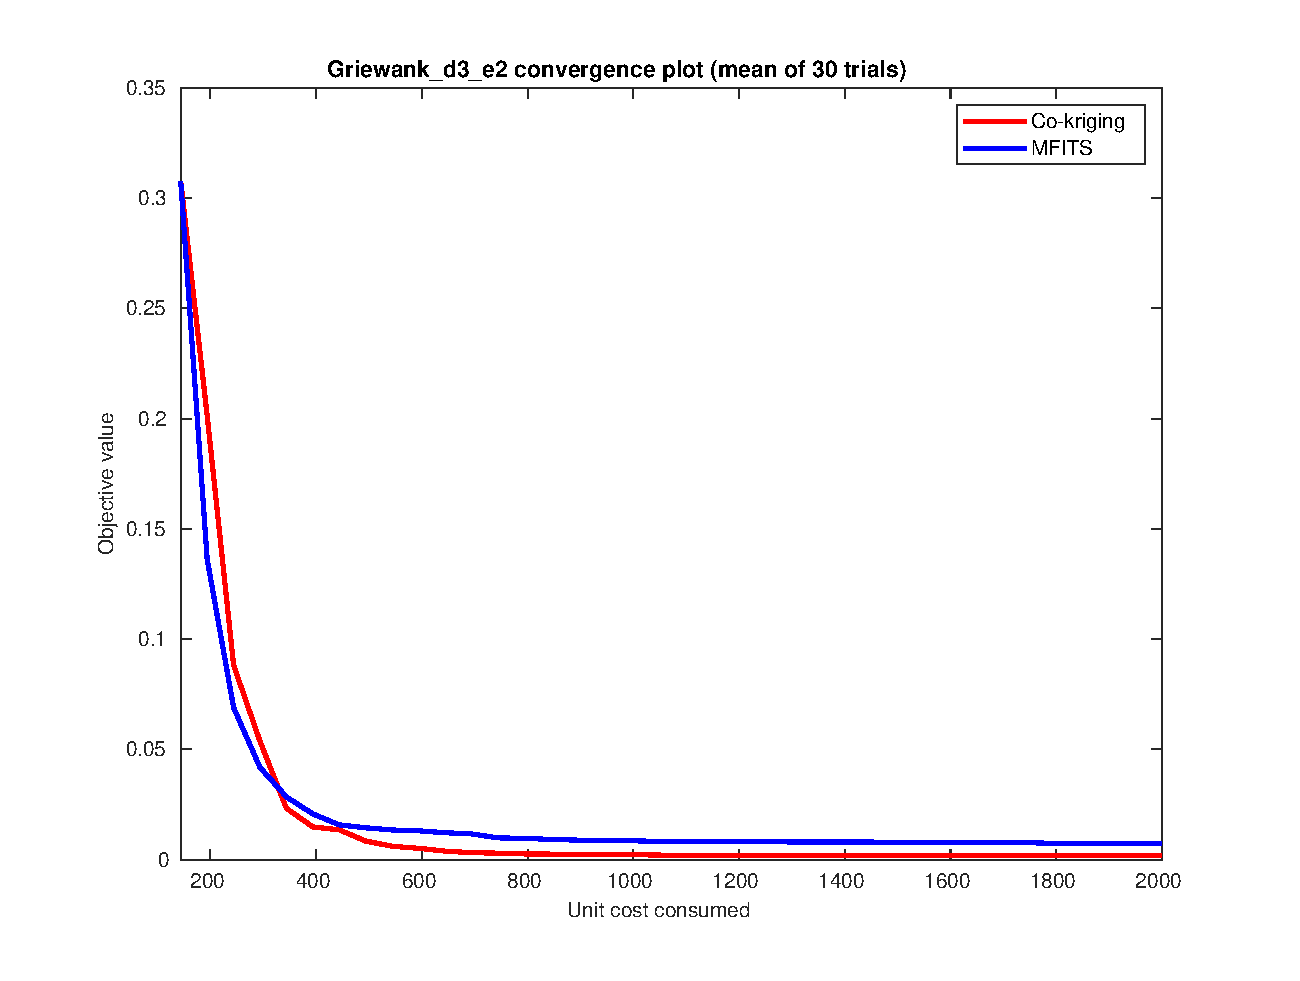
\includegraphics[width = 0.33\textwidth]{img/GW_d3_e2_conv_mean.eps}}
%   \subfloat[$Griewank_2\ (D=5)$\label{fig:gw25-conv}]{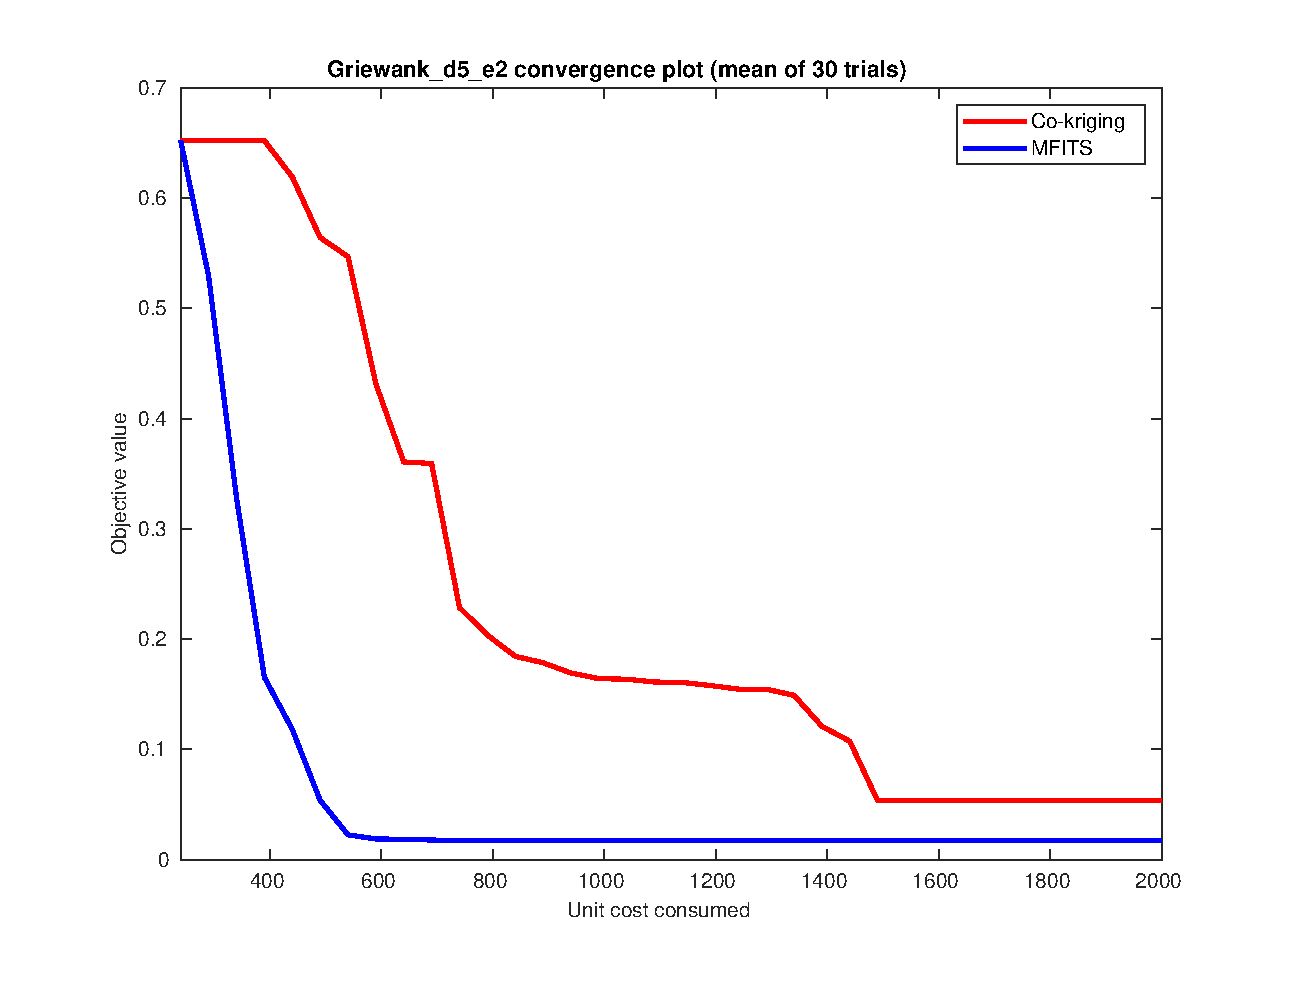
\includegraphics[width = 0.33\textwidth]{img/GW_d5_e2_conv_mean.eps}}
%   \subfloat[$Griewank_2\ (D=8)$\label{fig:gw28-conv}]{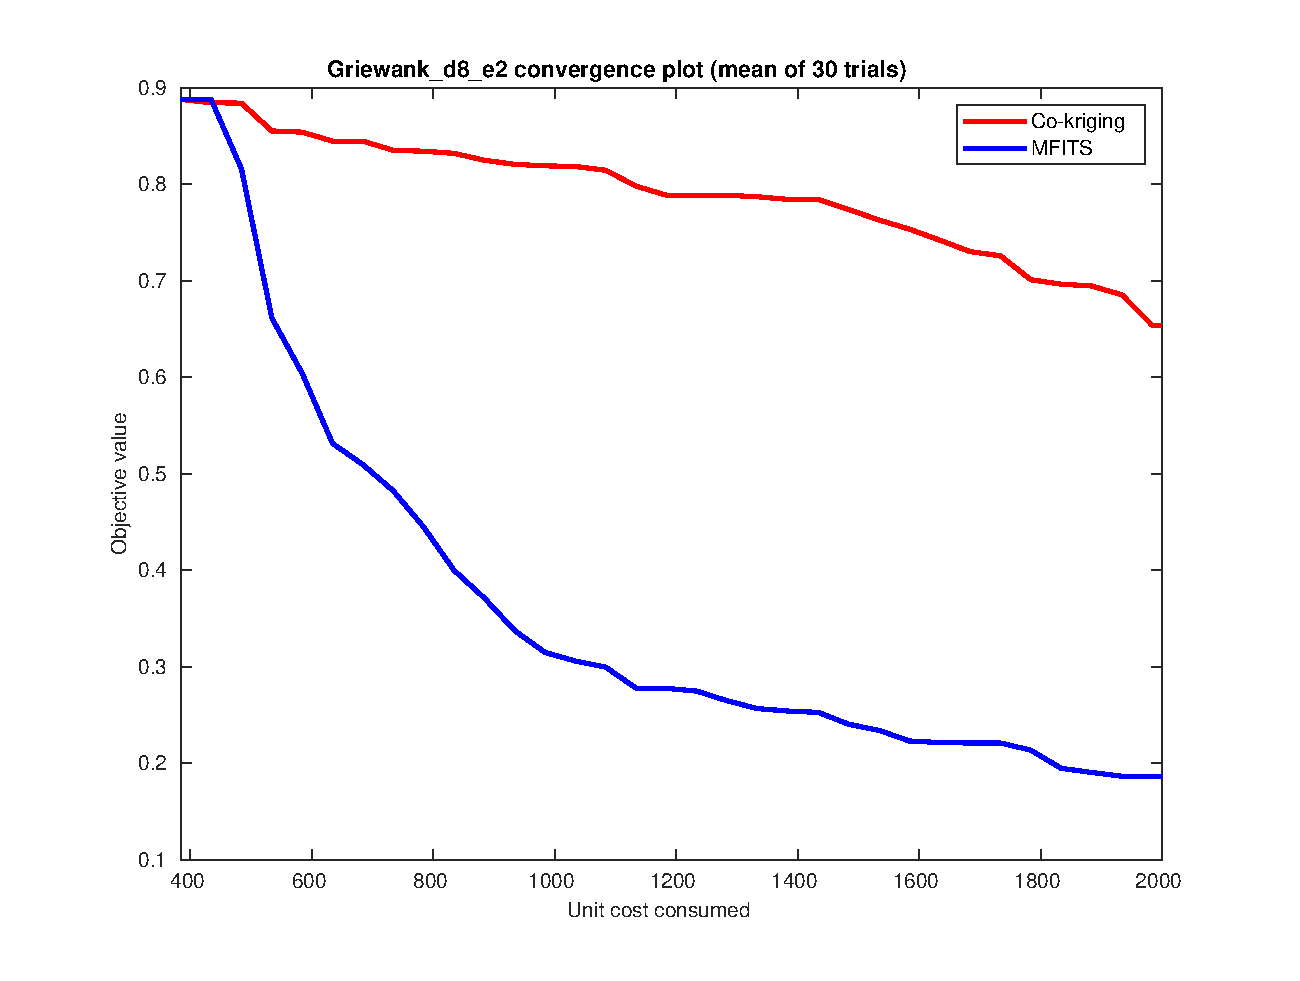
\includegraphics[width = 0.33\textwidth]{img/GW_d8_e2_conv_mean.eps}}\\
%   \subfloat[$Griewank_6\ (D=3)$\label{fig:gw63-conv}]{\includegraphics[width = 0.33\textwidth]{img/GW_d3_e6_conv_mean.eps}}
%   \subfloat[$Griewank_6\ (D=5)$\label{fig:gw65-conv}]{\includegraphics[width = 0.33\textwidth]{img/GW_d5_e6_conv_mean.eps}}
%   \subfloat[$Griewank_6\ (D=8)$\label{fig:gw68-conv}]{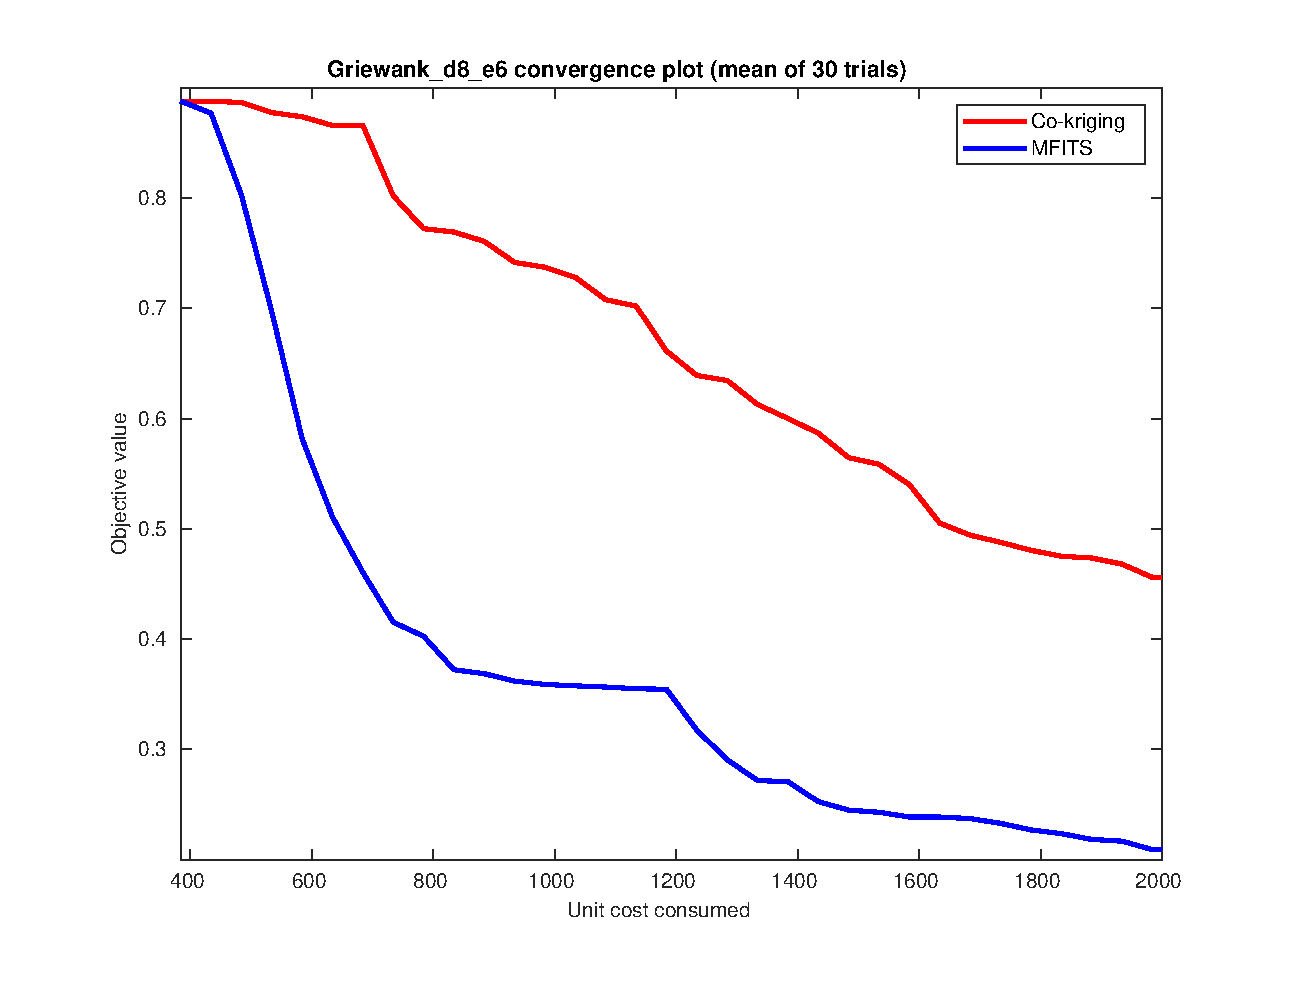
\includegraphics[width = 0.33\textwidth]{img/GW_d8_e6_conv_mean.eps}}
%   \caption{Mean convergence plots for $Griewank$ problem instance of dataset $B$, over 30 runs. \angus{will do pgfplots version}} 
%     \label{fig:set-b-conv}
% \end{figure*}
\begin{figure*}[h!]
  \centering
  \subfloat{\includegraphics{plots/obj_label.tikz}}%
  \addtocounter{subfigure}{-1}%
  \subfloat[$Griewank_2\ (D=3)$\label{fig:gw23-conv}]{\includegraphics[width = 0.28\textwidth]{plots/mfits/GW_d3_e2_plot.tikz}}
  \subfloat[$Griewank_2\ (D=5)$\label{fig:gw25-conv}]{\includegraphics[width = 0.28\textwidth]{plots/mfits/GW_d5_e2_plot.tikz}}
  \subfloat[$Griewank_2\ (D=8)$\label{fig:gw28-conv}]{\includegraphics[width = 0.28\textwidth]{plots/mfits/GW_d8_e2_plot.tikz}}\\
  \subfloat{\includegraphics{plots/obj_label.tikz}}%
  \addtocounter{subfigure}{-1}%
  \subfloat[$Griewank_6\ (D=3)$\label{fig:gw63-conv}]{\includegraphics[width = 0.28\textwidth]{plots/mfits/GW_d3_e6_plot.tikz}}
  \subfloat[$Griewank_6\ (D=5)$\label{fig:gw65-conv}]{\includegraphics[width = 0.28\textwidth]{plots/mfits/GW_d5_e6_plot.tikz}}
  \subfloat[$Griewank_6\ (D=8)$\label{fig:gw68-conv}]{\includegraphics[width = 0.28\textwidth]{plots/mfits/GW_d8_e6_plot.tikz}}
  \caption{Mean convergence plots for $Griewank$ problem instance of dataset $B$, over 30 runs. Blue and red colours indicate \AlgName{} and the co-kriging baseline, respectively.} 
    \label{fig:set-b-conv}
\end{figure*}

\subsection*{Discussion}
\begin{table}[h!]
\centering
\caption{Pairwise comparision of \AlgName{}, \motos{} and the base-line co-kriging algorithm using the MWW test.}\label{tab:mww-test}
% \begin{adjustbox}{width=\columnwidth}
\begin{tabular}{lrrrrrr} \toprule
& \multicolumn{3}{c}{Dataset $A$} & \multicolumn{3}{c}{Dataset $B$}\\
\cmidrule(lr){2-4} \cmidrule(lr){5-7} 
Algorithm & \multicolumn{1}{c}{Win}&\multicolumn{1}{c}{Draw} & \multicolumn{1}{c}{Loss}& \multicolumn{1}{c}{Win}&\multicolumn{1}{c}{Draw} & \multicolumn{1}{c}{Loss}\\ \midrule
%
\AlgName{} & \best{13} & 2 & 1 & \best{17} & 5 & 2 \\
Co-kriging & 9 & 2 & 5 & 10 & 8 & 6 \\
\motos{} & 0 & 0 & 16 & 0 & 5 & 19 \\   
%
\bottomrule
\end{tabular}
% \end{adjustbox}
\end{table}

Table~\ref{tab:mww-test} provides the results of a pairwise comparison of all three algorithms on both test suites, using the Mann-Whitney-Wilcoxon (MWW) statistical significance test~\cite{mann1947test}. This table clearly shows that \AlgName{} produces significantly better solutions than both \motos{} and the base-line co-kriging algorithm when considered across all problem instances and trials.

The results from both test suites suggest a similar pattern. For problems with few decision variables, there is very little difference between \AlgName{} and the base-line co-kriging algorithm. As the size of the problem increases, the convergence rate and performance of \AlgName{} improves over the simple co-kriging algorithm with the greatest improvements observed on the larger problem instances.

Although both algorithms contain the co-kriging technique as their principal constituent, the base-line algorithm uses a random sampling technique which gives it a disadvantage in problems with more decision variables, as it must cover an exponentially larger space with the same computational budget. By using the $LocalOCBA$ procedure to focus the sampling on areas of the search space that have been identified as promising, \AlgName{} can use its budget more efficiently to exploit these regions, which is evidenced by the faster convergence rates for larger problem sizes. %\hemant{Can this be visualized somehow on a couple of individual instances? Explicitly demonstrating it using some snapshot(s) will strengthen the this argument. Perhaps the explored solutions relative to the optimum in a 2D projected space (look up Sammon mapping, e.g.). The concentration of solutions in different areas can give some indicative illustration of how the search went and whether they focussed on the "right" areas. The plot will likely look very different for a low- vs high-dimensional problem, explaining the performance difference.}\angus{i will have a look into this and see if i can come up with something}

This claim is supported by the plots in Figure~\ref{fig:sammon}. This figure shows a Sammon mapping~\cite{sammon1969nonlinear} of the high- and low-fidelity evaluations made by all three algorithms on the three- and eight-dimensional instances of the $Griewank_2$ function from test suite $B$. The purpose of Sammon mapping is to project high dimensional data onto the two-dimensional plane, so it can be visualised, while maintaining similar ratios of euclidean distance ratios between all the points. 
\begin{figure*}[h!]
  \centering
  \quad \subfloat[\AlgName{} $(D=3)$\label{fig:sam-3d-mfits}]{\includegraphics[width = 0.28\textwidth]{plots/projections/GW_d3_e2_mfits_proj.tikz}}
  \subfloat[Co-kriging $(D=3)$\label{fig:sam-3d-cokrig}]{\includegraphics[width = 0.28\textwidth]{plots/projections/GW_d3_e2_cokrig_proj.tikz}}
  \subfloat[\motos{} $(D=3)$\label{fig:sam-3d-motos}]{\includegraphics[width = 0.28\textwidth]{plots/projections/GW_d3_e2_motos_proj.tikz}}\\
  \subfloat[\AlgName{} $(D=8)$\label{fig:sam-8d-mfits}]{\includegraphics[width = 0.28\textwidth]{plots/projections/GW_d8_e2_mfits_proj.tikz}}
  \subfloat[Co-kriging $(D=8)$\label{fig:sam-8d-cokrig}]{\includegraphics[width = 0.28\textwidth]{plots/projections/GW_d8_e2_cokrig_proj.tikz}}
  \subfloat[\motos{} $(D=8)$\label{fig:sam-8d-motos}]{\includegraphics[width = 0.28\textwidth]{plots/projections/GW_d8_e2_motos_proj.tikz}}
  \caption{Sammon mapping projection of samples onto the 2D plane for the Griewank function at $D=3$ and $D=8$. Points represent high- and low-fidelity samples, indicated by filled and un-filled circles, respectively; colour indicates solution quality, with red and blue being high and low, respectively; and the global optimum $\V{x}^*$ is indicated by the black cross.} 
    \label{fig:sammon}
\end{figure*}

Figures~\ref{fig:sam-3d-mfits},~\ref{fig:sam-3d-cokrig} and~\ref{fig:sam-3d-motos} give the Sammon mappings on the three-dimensional instance for \AlgName{}, co-kriging baseline and \motos{}, respectively. The Griewank function is highly multimodal, with many local optima and a single global optima, which is indicated by the multiple clusters of reddish coloured samples. The distribution of low-fidelity samples in Figures~\ref{fig:sam-3d-cokrig} and~\ref{fig:sam-3d-motos} is very similar and covers much of the search space, consistent with their policy of random sampling. The co-kriging baseline algorithm fared much better than \motos{} as it uses this information to build a model of the fitness landscape, which it searches globally, allowing it to locate the local optima on the left of the plot, and exploit that region with high-fidelity evaluations. In contrast, \motos{} is only able to evaluate candidate solutions in high-fidelity that it has already evaluated in low-fidelity; this means that, even though it sampled some solutions quite near to the global optimum by chance, it could not refine its search to focus on that area. The result is a set of high-fidelity evaluations which are multimodal, and possibly give a wider range of choices to a decision maker, but not necessarily of high quality. In~\cite{xu2016mo2tos}, up to 10,000 initial low-fidelity candidates were used for some problems which is well in-excess of the total computational budget of 2,000 low-fidelity-equivalent evaluations allowed in the experiments conducted here. As \motos{} must decide the finite set of solutions it can choose from \emph{a priori}, it heavily relies on chance as to whether that initial set contains promising candidates or not. This is particularly evident in the results obtained for larger instances of test suite $A$, where the limited budget for initial samples must be spread over a high-dimensional space.

Illustrated by Figure~\ref{fig:sam-3d-mfits}, it can be seen that \AlgName{} identified the same local optima as the co-kriging baseline; however, it did so with a more efficent use of its computing budget. Both algorithms started with exactly the same initial populations, but it is clearly shown in the plots that \AlgName{} takes a much more targeted approach to its low-fidelity sampling than the co-kriging baseline or \motos{}. Another interesting thing to note about this instance is that, although the co-kriging algorithm got stuck in a local optima; towards the very end of the search, \AlgName{} was able to escape this local optima and find a new region to exploit which was much closer to the global optimum, using the mechanism described by Equation~\ref{eq:epsilon} --- had there been more budget allowed, it is likely that \AlgName{} would have continued to exploit this region, eventually finding the global optimum. 

In the three-dimensional case, the ``scatter-gun'' approach to low-fidelity sampling adopted by the co-kriging baseline algorithm and \motos{} is not especially detrimental. The entire space can be covered reasonably effectively with the allocated budget and it does not matter if some of the evaluations are wasted on regions of the search space that are not very productive. The eight-dimensional case depicted in Figures~\ref{fig:sam-8d-mfits},~\ref{fig:sam-8d-cokrig} and~\ref{fig:sam-8d-motos} tells a much different story, however. Here, the search space is exponentially larger and the fixed budget must be spent more thriftily. Figures~\ref{fig:sam-8d-cokrig} and~\ref{fig:sam-8d-motos} show that there is not much difference between \motos{} and the co-kriging baseline; \motos{} takes a one-shot, ``hit-and-hope'' approach, and the co-kriging baseline is unable to garner enough information from randomly sampling to construct a useful model of the search space. 

It is in these higher-dimensional spaces where the targeted approach to low-fidelity sampling taken by \AlgName{}, illustrated in Figure~\ref{fig:sam-8d-mfits}, comes into its own. After spending some time focusing in a less productive area (indicated by the denser pattern of low-fidelity samples to the upper right), the search finally manages to locate a region which it can exploit to produce better quality solutions. This is where the guided DE process described in Section~\ref{sec:method} is important; because even though there are so many directions to get lost in, newly constructed candidate solutions are always pushed towards the region that has proven most fruitful so far.

% Finally, although the numerical results and convergence plots do indicate that there is not a significant difference between the performance of \AlgName{} and the base-line co-kriging algorithm on the smaller instances; it is worth noting that for three out of four of these instances, the co-kriging baseline did perform slightly better on average. One possible explanation for this is that the $LocalOCBA$ procedure makes \AlgName{} more greedy, and therefore more likely to become trapped in local optima --- especially for multimodal instances like the Griewank problem. In these smaller instances, the random sampling of the base-line co-kriging algorithm is not as much of a disadvantage and it is more likely to come across good areas of the search space by chance.